\documentclass[11pt,a4paper]{report}
\usepackage[utf8]{inputenc}
\usepackage[french]{babel}
\usepackage[T1]{fontenc}
\usepackage{amsmath}
\usepackage{amsfonts}
\usepackage{amssymb}
\usepackage{xcolor}

\usepackage{geometry}
\geometry{hmargin=2.5cm,vmargin=1.5cm}
\usepackage{wasysym}
\usepackage{graphicx}

\author{Mathieu Sarrat}
\title{LP5 - Phénomènes interfaciaux impliquant des fluides}

\makeatletter
\renewcommand{\thesection}{\@arabic\c@section}
\makeatother


\begin{document}
\maketitle

\subsection{Pré-requis}
\begin{itemize}
	\item Thermodynamique
	\item Mécanique des fluides
\end{itemize}

\subsection{Objectifs}
\begin{itemize}
	\item Introduction de la notion de tension de surface
	\item Applications : ascension capillaire, mouillage
	\item Mesure d'un coefficient de tension de surface
\end{itemize}

\newpage
\section*{Introduction}

\begin{itemize}
	\item On dit souvent qu'un liquide adopte la forme du récipient qui le contient : 
	ce n'est pas tout à fait exact.\\ 
	(Gouttes d'eau sur des feuilles)\\
	(Diapo de billes de mercure de différentes tailles) : compétition entre deux grands effets (une tendance à minimiser la surface libre du liquide, une tendance à étaler le liquide, d'autant plus prononcée que la masse de liquide est importante).\\
	
	\item Les phénomènes interfaciaux, c'est à dire se produisant à la surface de séparation entre deux phases fluides (deux liquides non-miscibles, un liquide et un gaz), sont étudiés depuis longtemps : Léonard de Vinci avait déjà remarqué l'ascension surprenante d'un liquide contenu dans un tube vertical suffisamment étroit [Photos ou schéma, au pire].\\ 
\end{itemize}

\section{Tension de surface}

\subsection{Mise en évidence}

\textcolor{red}{Manip qualitative si possible :} cadre + bain d'eau savonneuse + tige fine. Placer la tige sur le cadre pour délimiter deux espaces. Plonger légèrement le cadre dans un bain d'eau savonneuse pour arracher une pellicule de fluide qui va se loger dans les deux espaces. Crever l'une des deux pellicules et observer la seconde attirer la tige mobile vers elle. 

\textit{Eau savonneuse car tension de surface plus faible que l'eau : plus facile de générer et stabiliser une pellicule de grande taille si la tension de surface (liée à l'intensité de la force de rappel) est faible.}

\subsection{Interprétation macroscopique}

Modélisons macroscopiquement ce que nous venons de voir, nous allons nous appuyer sur la situation suivante : un cadre rectangulaire dont l'un des côtés est mobile (de longueur $L_0$ délimite une lame de liquide de surface $A$. On repère un point M du côté mobile et on exerce une force de traction sur ce côté pour augmenter la surface du film fluide, et donc pour augmenter la surface $A$ de fluide en contact avec l'air.\\

\begin{figure}[h!]
\begin{center}
	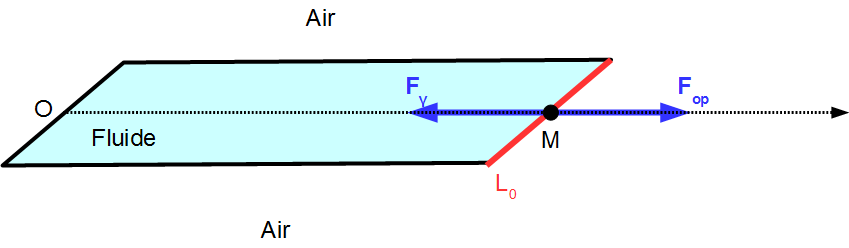
\includegraphics[scale = 0.5]{force_superficielle.png} 
	\label{fig:force_superficielle}
\end{center}
\end{figure}

	\subsubsection{Force de tension superficielle}	
	
Le fluide exerce une réaction $\bold{F}_\gamma$ sur la partie mobile du cadre : force de tension superficielle. Elle tend à réduire l'aire de l'interface, en essayant de ramener le cadre vers sa position initiale.
	
La force de tension superficielle qui s'exerce sur un élément $d\ell$ du côté mobile est :
\begin{itemize}
	\item \textbf{tangente à l'interface},
	\item perpendiculaire à l'élément de longueur sur lequel elle s'exerce,
	\item proportionnelle à $d\ell$.
\end{itemize}

Ainsi, la force de tension de surface totale (il y a en fait deux interfaces, entre le fluide et l'air au-dessus, et entre le fluide et l'air au-dessous) exercée sur le côté mobile du cadre s'écrit :
\begin{equation}
	\bold{F}_\gamma = - 2 \left(\gamma L_0\right) \bold{e}_x.
\end{equation}

Le coefficient de proportionnalité $\gamma$ est appelé \textbf{coefficient de tension superficielle} et s'exprime en $\text{N}.\text{m}^{-1}$.

La tension de surface dépend de la nature des fluides en contact, mais aussi de la température. Pour des variations de température modérées, on peut écrire
\begin{equation}
	\gamma(T) = \gamma(T_0)\left[1 - b(T-T_0)\right],
\end{equation}
où $b$ est un coefficient valant entre $10^{-2}$ et $10^{-1}\;\text{K}^{-1}$. \textbf{La tension de surface diminue avec la température}.

On donne quelques valeurs de $\gamma$ pour une interface liquide/air :
\begin{center}
\begin{tabular}{|c|c|c|c|c|}
  \hline
  	Corps & $\gamma$ (mN.$\text{m}^{-1}$) \\
  \hline
  \hline
  	Eau pure 293 K & 73 \\
  \hline
  	Eau pure 323 K & 68 \\
  \hline
	Eau savonneuse 293 K & 25 \\
  \hline
  	Glycérine 290 K & 65 \\
  \hline
  	Mercure 291 K  & 500\\
  \hline
  	\'Etain fondu 532 K  & 526\\
  \hline
\end{tabular}
\end{center}

Le cas de l'eau savonneuse est intéressant : le coefficient $\gamma$ est divisé par 3 grâce à l'ajout de savon à température ambiante. Le savon est un tensioactif (ou surfactant) : sa présence à l'interface abaisse la tension de surface entre les fluides.

	\subsubsection{Définition thermodynamique}

Pour augmenter l'aire de l'interface, il a fallu exercer une certaine force, $\bold{F}_\text{op} = - \bold{F}_\gamma$. On a fourni \textbf{via cette force} $\bold{F}_\text{op}$ de l'énergie sous forme de travail au fluide :
\begin{equation}
	\boxed{\delta W = - \bold{F}_\gamma \cdot d\bold{r} = \gamma 2 L_0 d\ell \equiv \gamma dA}.
\end{equation} 
En dimension, le coefficient de tension superficielle correspond à une \textbf{énergie par unité de surface}.\\

Pour un corps pur de volume $V$, l'énergie interne $U$ est une fonction des variables $S$ et $V$. Une interface est un volume dont l'une des dimensions spatiales est faible devant les deux autres : $V = A\epsilon$ ou $\epsilon$ est négligeable. Ainsi, $U = U(S,A)$. Pour une transformation quelconque, la variation d'énergie interne \textbf{de l'interface} s'écrit :
\begin{equation}
	dU = \left(\frac{\partial U}{\partial S}\right)_A dS + \left(\frac{\partial U}{\partial A}\right)_S dA = T dS + \left(\frac{\partial U}{\partial A}\right)_S dA.
\end{equation}
Or, pour une transformation réversible, le Premier Principe implique :
\begin{equation}
	dU = \delta Q + \delta W = \delta Q + \gamma dA = TdS + \gamma dA,
\end{equation} 
de sorte que
\begin{equation}
	\boxed{\gamma \equiv \left(\frac{\partial U}{\partial A}\right)_S}.
\end{equation}

En introduisant l'énergie libre $F = U - TS$ on obtient
\begin{equation}
	dF = -SdT + \gamma dA.
\end{equation}
Si la transformation s'effectue à température constante,
\begin{equation}
	dF = \gamma dA.
\end{equation}
Pour une interface homogène, $\gamma dA = d\left(\gamma A\right)$, d'où
\begin{equation}
	F = \gamma A.
\end{equation}

Le travail \textbf{des forces de tension de surface} s'écrit $\delta W_\gamma = - \delta W = - d\left(\gamma A\right) \equiv - dE_p$, où $E_p$ est une énergie potentielle. Cela implique $F = E_p$. L'énergie libre s'identifie à l'énergie potentielle des forces de tension superficielle.\\

Une structure stable par rapport à ces forces est donc une structure pour laquelle la surface est minimale compte tenu des contraintes imposées au système (par exemple la gravité ou la pression). [Photo du capitaine Haddock et de son whisky + commentaires (apesanteur), la sphère est la surface d'aire minimale pour un volume donné].

\subsection{Interprétation microscopique}

Dans un liquide, les interactions entre particules (atomes ou molécules) sont importantes et ne peuvent pas être négligées : interactions de Van der Waals, liaisons hydrogène, liaisons métalliques (métal liquide comme le mercure). \textbf{La tension de surface est la résultante des forces de cohésion internes s'exerçant entre les molécules du fluide}.

\begin{figure}[h!]
\begin{center}
	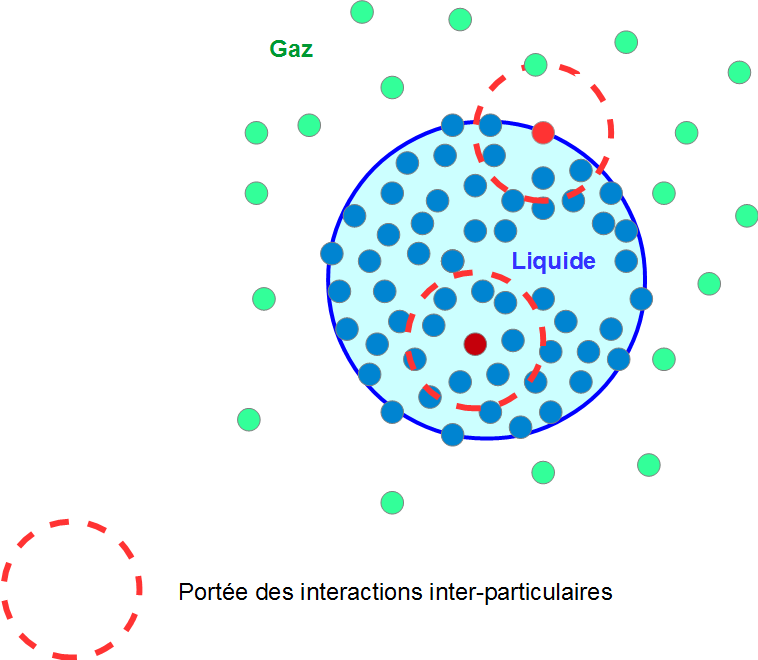
\includegraphics[scale = 0.5]{tension_micro.png} 
	\label{fig:tension_micro}
\end{center}
\end{figure}

Au cœur du fluide, les forces d'interaction exercées par chaque molécule sont globalement équilibrées par celles qu'exercent les molécules voisines. \'A proximité d'une interface, par exemple avec du vide ou un gaz très dilué, il n'y a plus cet équilibre. C'est là l'origine des forces de tension superficielle.

\begin{figure}[h!]
\begin{center}
	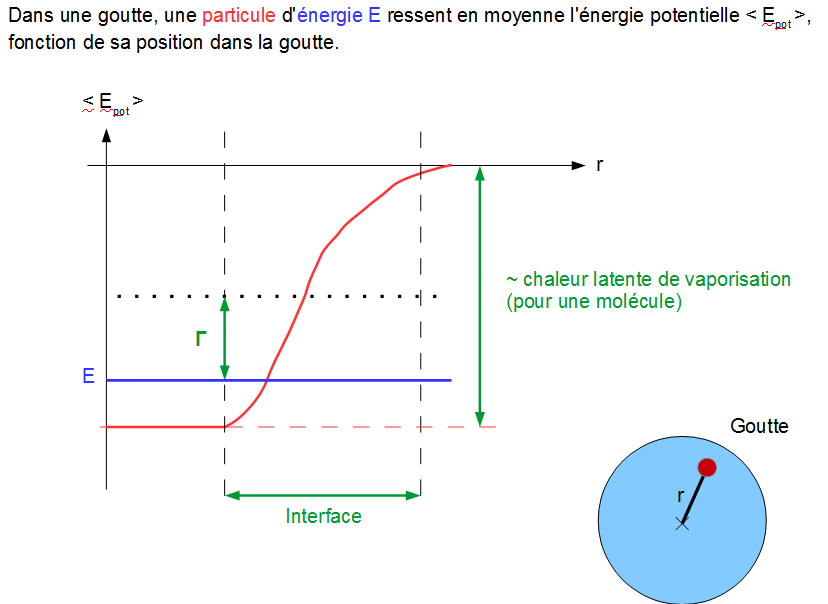
\includegraphics[scale = 0.5]{interp_micro.png} 
	\label{fig:interp_micro}
\end{center}
\end{figure}

Une particule de la goutte se trouve dans le puits d'énergie potentielle (généré par les interactions inter-particulaires) représenté en figure \ref{fig:interp_micro}, fonction de sa position par rapport au centre de la goutte.\\

Soit $\Gamma$ l'énergie à apporter à une molécule pour l'amener à la surface. Essayons d'interpréter microscopiquement le raisonnement thermodynamique présenté auparavant. Pour amener $N$ particules à la surface (et augmenter l'aire de celle-ci de $dA$), on doit fournir en moyenne le travail $\delta W = N\Gamma$. Si on note $a_0$ l'aire moyenne occupée par une particule à la surface,
\begin{equation}
	N = \frac{dA}{a_0}
\end{equation}
et donc 
\begin{equation}
	\delta W = \Gamma \frac{dA}{a_0} \equiv \gamma dA,\quad\text{d'où}\quad \gamma = \frac{\Gamma}{a_0}
\end{equation}
le coefficient de tension de surface, en $J.\text{m}^{-2}$ (ou en $N.\text{m}^{-1}$).\\

L'énergie $\Gamma$ dépend de l'énergie cinétique de la particule. Sa valeur moyenne dépend donc de la température : \textbf{plus la température sera grande, plus l'énergie cinétique d'une particule sera importante (en moyenne) et plus il lui sera facile d'atteindre la surface} (l'énergie à fournir $\Gamma$, et donc $\delta W$ sera plus faible). On arrive ainsi à voir pourquoi $\gamma$ diminue avec la température.\\

La valeur de $\gamma$ dépend aussi de la nature des liaisons physiques en jeu : la forte tension superficielle des métaux liquides (mercure, étain fondu) est liée à la forte valeur des énergies associées aux liaisons métalliques (quelques eV pour une liaison). Lorsque la cohésion du liquide est assurée par les interactions de Van der Waals, la valeur de $\gamma$ chute, ces interactions étant beaucoup plus faibles.
 
\subsection{Mesure d'un coefficient de tension de surface}

Méthode par arrachement de Lecomte de Noüy : mise au point par le biologiste français Lecomte de Noüy au début du $\text{XX}^\text{e}$ siècle.\\

\textbf{Principe 1 :}
\begin{itemize}
	\item Plonger un anneau (rayon extérieur $r_e$, rayon intérieur $r_i$) de masse $m$ dans un fluide.
	\item Arracher l'anneau de la surface avec un dynamomètre.
	\item Mesurer la force minimale requise pour arracher l'anneau (dynamomètre) : on en déduit la tension de surface.
\end{itemize}

Bilan des forces appliquées \textbf{à l'anneau} avant rupture ($\bold{e}_z$ verticale ascendante) :
\begin{equation}
	\bold{0} = \bold{F}_\text{op} + m\bold{g} + \bold{F}_\gamma,
\end{equation}
avec $\bold{F}_\gamma = -2\pi r_i \gamma \bold{e}_z - 2\pi r_e \gamma \bold{e}_z \equiv - 4\pi\gamma r \bold{e}_z$ où
\begin{equation}
	r = \frac{r_e + r_i}{2}.
\end{equation}
On trouve
\begin{equation}
	\gamma = \frac{F_\text{op} - mg}{4\pi r}.\\
\end{equation}

\textbf{Principe 2 :} avec une balance au lieu d'un dynamomètre.
\begin{itemize}
	\item Placer sur la balance : récipient + liquide + anneau. Masse $m_l$ lue sur la balance.
	\item Tirer sur l'anneau. La masse diminue au fur et à mesure qu'on tire. Relever la valeur $m_a$ juste avant la rupture.
	\item Relever la valeur de masse $m_r$ après rupture. Normalement $m_r = m_l$.
\end{itemize}

Bilan des forces \textbf{appliquées au fluide} avant rupture :
\begin{equation}
	\bold{0} = \bold{R}_\text{a} + m_l\bold{g} + \bold{F}_\gamma,
\end{equation}
où la force de traction $\bold{F}_t$ exercée sur le fluide est l'opposé de la force de tension de surface exercée par le fluide sur l'anneau. On a donc cette fois-ci dirigée vers le haut et s'écrit $\bold{F}_t = -\bold{F}_\gamma = 4\pi\gamma r \bold{e}_z$. La force de réaction de la balance est interprétée par celle-ci comme le poids d'une masse apparente : $\bold{R}_a = - m_a \bold{g}$. En projetant selon Oz ($\bold{g} = - g\bold{e}_z$) :
\begin{equation}
	0 = (m_a - m_l) g + 4\pi\gamma r,
\end{equation}
d'où :
\begin{equation}
	\gamma = \frac{(m_l - m_a)g}{4\pi r}.
\end{equation}

Mesurer valeur et comparer à la littérature si possible. Discuter les erreurs \textcolor{red}{(à identifier durant la préparation)} :
\begin{itemize}
	\item Ne pas toucher l'anneau avec les doigts : ça graisse (tensioactif) et ça va diminuer la valeur mesurée).
\end{itemize}

\newpage
\section{Description de l'interface entre deux fluides}

Maintenant que nous avons défini les forces de tension de surface, voyons comment introduire ces effets dans la théorie de la mécanique des fluides.

\subsection{Conditions de bord dans la résolution de l'équation de Navier-Stokes}

Rappelons l'équation de Navier-Stokes pour un écoulement incompressible de fluide visqueux :
	\begin{equation}
		\rho\left(\frac{\partial\bold{v}}{\partial t}+\left(\bold{v}\cdot\bold{\text{grad}}\right)\bold{v}\right)=\rho\bold{g}-\bold{\text{grad}}(p)+\eta\Delta\bold{v},
	\end{equation}	

Les effets de tension de surface n'apparaissent pas dans cette équation : comme ils ne sont importants qu'à la surface du fluide, on les introduit via les conditions de bord.

Ces conditions, applicables à la frontière du domaine occupé par le fluide, sont :
\begin{itemize}
	\item \textcolor{red}{contact entre un fluide et un solide} : égalité entre la vitesse du solide et la vitesse du fluide au contact du solide (continuité de la vitesse et imperméabilité).
	
	\item \textcolor{red}{contact entre deux fluides non-miscibles} :
		\begin{itemize}
			\item continuité de la vitesse à l'interface (cf. ci-dessus),
			\item continuité des contraintes tangentielles (forces de viscosité) et normales (forces de pression) à l'interface.
		\end{itemize}
\end{itemize}

La continuité des contraintes de pression ne correspond \textbf{pas toujours} à \textbf{une simple égalité de la pression des deux fluides de part et d'autre de l'interface}, comme on le fait parfois un peu naïvement : la courbure de l'interface et le coefficient de tension de surface interviennent. La relation décrivant cette condition de bord est la \textbf{Loi de Laplace}.

\subsection{Loi de Laplace}

\subsubsection{Cas simple : interface sphérique entre deux milieux}

Interface sphérique de rayon $R$ entre deux fluides : goutte sphérique (1) immergée dans un autre fluide (2).

Point de vue thermodynamique. On considère le système suivant :
\begin{itemize}
	\item Fluide 1, de volume $V = 4/3 \pi R^3$
	\item Interface de surface $A = 4\pi R^2$ entre les deux fluides.\\
\end{itemize}

On recherche l'équilibre de cette goutte dans l'atmosphère, considéré comme un thermostat de température $T_0$ et un réservoir de volume à la pression $p_0$. On néglige la pesanteur ainsi que l'évaporation à la surface de la goutte : le système est supposé fermé (pas d'échange de matière avec l'atmosphère).\\

Température et pression extérieures sont fixées, l'équilibre du système est donnée par le minimum de la fonction \textbf{enthalpie libre externe}
\begin{equation}
	\boxed{G_0 = U - T_0 S + p_0 V},
\end{equation} 
$U$, $S$ et $V$ étant les variables internes du système. On a donc
\begin{equation}
	dG_0 = dU - T_0 dS + p_0 dV,
\end{equation}
avec
\begin{equation}
	dU = dU_1+dU_\text{int}=\left(T_1 dS_1-pdV\right)
	+\left(T_\text{int}dS_\text{int}+\gamma dA\right),
\end{equation}
d'où
\begin{equation}
	dG_0 = \left(T_1 - T_0\right)dS_1 + \left(T_\text{int} - T_0 dS_\text{int}\right)
	+\left(p_0 - p\right)dV + \gamma dA.
\end{equation}
Volume du fluide 1 et aire de l'interface ne sont pas des variables indépendantes, car
\begin{equation}
	dV = 4\pi R^2 dR \quad\text{et}\quad dA = 8\pi R dR, 
\end{equation}
d'où
\begin{equation}
	dG_0 = \left(T_1 - T_0 \right)dS_1 
	+ \left(T_\text{int} - T_0 \right)dS_\text{int}
	+ 4\pi R^2 \left(p_0 - p + 2\frac{\gamma}{R}\right) dR = 0
\end{equation}
la dernière égalité étant vraie à l'équilibre. Il en découle, $S_1$, $S_\text{int}$ et $R$ étant indépendantes,
\begin{equation}
	T_1 = T_\text{int} = T_0
\end{equation}
et la \textbf{loi de Laplace pour une interface sphérique} :
\begin{equation}
	\boxed{p_1 - p_2 = 2\frac{\gamma}{R}}.
\end{equation}

L'intérieur de la goutte est donc en surpression par rapport à l'extérieur.

\subsubsection{Cas général}

En un point d'une interface de forme quelconque :
\begin{equation}
	\boxed{p_1 - p_2 = \gamma \underbrace{\left(\frac{1}{R} 
	+ \frac{1}{R'}\right)}_{\displaystyle{\equiv C}}}.
\end{equation}

Dans cette expression :
\begin{itemize}
	\item $p_1$ est la pression côté concave
	\item $p_2$ est la pression côté convexe
	\item $R$ et $R'$ sont les rayons de courbure principaux $R$ et $R'$ au point considéré. $C$ est la courbure moyenne locale en ce point.\\
\end{itemize}

$R$ et $R'$ sont algébriques : positifs si le centre de courbure est placé dans le fluide (1) (fluide 1 côté concave, fluide 2 côté convexe).\\

On retrouve bien le cas de la symétrie sphérique en posant $R = R'$. Plus la courbure est faible, plus la différence de pression de part et d'autre de l'interface l'est aussi.

\subsection{Surpression dans une bulle de savon}

Savon constitué de molécules amphiphiles, c.a.d comprenant :
\begin{itemize}
	\item une partie hydrophile (la tête polaire, aime l'eau)
	\item une partie hydrophobe/lipophile (la queue, aime le gras, chaine carbonée)
\end{itemize}

Bulle de savon : deux interfaces sphériques eau savonneuse/air concentriques [SCHEMA]

L'épaisseur d'eau savonneuse étant faible, on a 
\begin{equation}
	p_1 - p_1' = 2\frac{\gamma}{R} \quad\text{et}\quad p_1' - p_2 = 2\frac{\gamma}{R},
\end{equation}
d'où
\begin{equation}
	p_1 - p_2 \equiv \Delta p = 4\frac{\gamma}{R}.
\end{equation}

Cette surpression $\Delta p$ est d'autant plus grande que la bulle est petite.


\newpage
\section{Phénomènes interfaciaux}

\subsection{Mouillage d'une surface}

Soit une goutte immobile sur un support liquide : photos de gouttes d'eau sur du verre et sur un support hydrophobe. Le liquide ne s'étale pas totalement : il y a un équilibre mécanique. On dit que la goutte \textbf{mouille} plus ou moins la surface solide.\\

Représentons schématiquement ce que l'on voit.\\

\begin{figure}[h!]
\begin{center}
	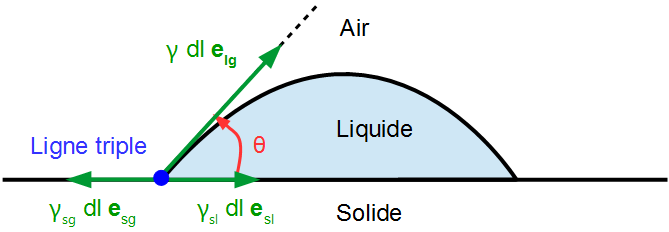
\includegraphics[scale = 0.5]{mouillage.png} 
	\label{fig:mouillage}
\end{center}
\end{figure}

Lorsqu'une goutte mouille une surface solide, il y a trois interfaces différentes : entre la goutte et l'air, entre l'air et le solide, entre la goutte et le solide. Il existe une ligne, la \textbf{ligne triple}, intersection de ces trois interfaces. L'angle $\theta$ est appelé \textbf{angle de mouillage} est l'angle que fait le plan tangent à la surface de la goutte avec le plan du support. Un élément $d\bold{\ell}$ de cette ligne est soumis à trois forces de tension superficielle, perpendiculaires à $d\bold{\ell}$ :
\begin{itemize}
	\item la force $\bold{F}_{\gamma,lg} = \gamma_\text{lg} d\ell \bold{e}_\text{lg} = \gamma d\ell \bold{e}_\text{lg}$ tangente à l'interface liquide/gaz, faisant l'angle $\theta$ avec l'axe $\text{Ox}$,
	\item la force $\bold{F}_{\gamma,sl} = \gamma_\text{sl} d\ell \bold{e}_\text{sl}$ tangente à l'interface solide/liquide, orientée selon $\text{Ox}$,
	\item la force $\bold{F}_{\gamma,sg} = \gamma_\text{sg} d\ell \bold{e}_\text{sg}$ tangente à l'interface solide/gaz, orientée selon $-\text{Ox}$.\\
\end{itemize}
Les forces de tension de surface sont parallèles à l'interface, perpendiculaires à la ligne sur laquelle elles s'exercent.
 
\'A l'équilibre, les forces de tension superficielle se compensent selon la direction $Ox$ :
\begin{equation}
	\left(\gamma \text{cos}\;\theta + \gamma_\text{sl} - \gamma_\text{sg}\right) d\ell = 0
\end{equation}
d'où la \textbf{Relation d'Young} :
\begin{equation}
	\text{cos}\;\theta = \frac{\gamma_\text{sg} - \gamma_\text{sl}}{\gamma}
\end{equation}

On peut introduire le \textbf{paramètre d'étalement} $S$ :
\begin{equation}
	\boxed{S \equiv \gamma_\text{sg} - \left(\gamma_\text{sl} + \gamma\right)},
\end{equation}
auquel cas la relation d'Young s'écrit
\begin{equation}
	\boxed{\text{cos}\;\theta = 1 + \frac{S}{\gamma}}.
\end{equation}

Compte tenu de l'expression de la relation d'Young, un paramètre d'étalement $S > 0$ implique l'absence d'équilibre et donc un mouillage complet de la surface : il \textbf{est énergétiquement favorable d'étaler le liquide autant que possible}. Au contraire, un paramètre d'étalement $S \leq 0$ implique un mouillage partiel :
\begin{itemize}
	\item si $\theta$ est aigu, la goutte \textbf{mouille beaucoup} la surface solide : elle a tendance à s'étaler beaucoup;
	\item si $\theta$ est obtus, la goutte \textbf{mouille peu} la surface solide. C'est le cas de la goutte d'eau sur le support hydrophobe, ou d'une goutte de mercure sur du verre.\\ 
\end{itemize}

On parle de \textbf{mouillage fort} lorsque $\theta \simeq 0$ : le liquide s'étale totalement sur la surface solide. Cette situation est recherchée lorsqu'on souhaite entretenir un tissu, par exemple. L'utilisation de substances tensioactives dans l'eau permet à l'eau de mieux imbiber le linge, améliorant l'efficacité du nettoyage.\\

On parle de mouillage faible ou mouillage nul lorsque $\theta \simeq 180$. La goutte n'est en contact avec la surface que par un point. Les forces de tension superficielles sont capables de compenser le poids, ce qui explique la faculté de certains insectes à marcher sur l'eau [Diapo photo]. Les acides gras (hydrophobes) sécrétés par certains oiseaux, comme les canards, imbibent leur plumage et leur permet de rester au sec. Pour rendre un tissu imperméable, on l'enduit d'une substance tensioactive. Pour faciliter leur collecte en cas de problème, on peut chercher à réduire le mouillage des produits pétroliers accidentellement répandus sur la mer.\\

\subsection{Capillarité}

Nous allons discuter d'une autre grande catégories de phénomènes directement liés aux forces de tension superficielle : l'ascension de liquides le long de parois solides verticales (sucre trempé dans du café, sève dans les arbres). Cette ascension se fait par capillarité.\\

\textcolor{green}{Manip :} récipient contenant de l'eau, on plonge un tube cylindrique de rayon $r$ ouvert aux deux extrémités dans le récipient et on mesure la hauteur de l'eau dans ce tube. On mentionne également la présence d'un ménisque : la surface libre du liquide est courbe à proximité de la paroi. Montrer que l'eau monte d'autant plus haut que le tube est fin. Mentionner qu'avec du mercure, le ménisque est de concavité opposée et que le niveau de mercure dans le tube est plus bas que le niveau de mercure hors du tube [Schémas ou photos pour le mercure]. Relier le type de concavité du ménisque pour l'eau et le mercure au mouillage du verre par ces liquides : \textbf{l'eau mouille le verre, le mercure ne le mouille pas}.\\

Schématisons cette situation \textcolor{red}{(voir diapo)} : le fluide est au repos dans la colonne. Le gradient de pression dans le fluide est de nature hydrostatique
\begin{equation}
	p(h) - p_\text{atm} = -\rho g h.
\end{equation} 
On applique la \textbf{loi de Laplace au niveau du ménisque, supposé sphérique}
\begin{equation}
	p_\text{atm} - p(h) = \frac{2\gamma}{R} = \frac{2\gamma \text{cos}\;\theta}{r},
\end{equation}
$r$ étant le rayon du cylindre.\\
On trouve alors la \textbf{loi de Jurin} reliant la hauteur de la colonne à la tension de surface et aux caractéristiques du tube.
\begin{equation}
	\boxed{h = 2\frac{\gamma}{\rho g} \frac{\text{cos}\;\theta}{r}}.
\end{equation}
Ce type d'expérience permet de mesurer $\gamma$.\\

\textbf{Remarque sur l'hypothèse de sphéricité du ménisque :}\\
Dans un tube circulaire, le ménisque est sphérique si sa courbure est la même en tout point. La loi de Laplace implique alors que la différence de pression entre l'air et le liquide est partout la même. L'air étant beaucoup moins dense que le liquide, cela signifie plus précisément que la pression dans le liquide juste au-dessous du ménisque est homogène.\\

Cela n'est évidemment pas rigoureusement le cas puisque le bord du ménisque (la ligne triple) est situé à une distance $\delta$ au-dessus du centre du ménisque. On montre toutefois que l'hypothèse est satisfaisante si $\delta \ll h$.





\subsubsection*{Longueur capillaire}

Les effets de capillarité dont nous venons de discuter sont liés à la courbure des interfaces et sont importants lorsqu'on s'intéresse à de petites échelles de longueur : plus le tube cylindrique est étroit, plus l'eau monte haut. On comprend intuitivement que pour des objets de grande taille, ces effets puissent être masqués par l'influence des forces en volume, comme la gravité. En témoigne la forme de gouttes de mercure de masses croissantes déposées sur une plaque de verre : plus la goutte est grosse, plus elle s'étale, alors que la nature des interfaces est la même pour chaque goutte. La question qui découle de ce constat est la suivante : quelle est la taille typique du système en deçà de laquelle les effets de tension de surface deviennent incontournables dans la modélisation ?\\

Si on observe la loi de Jurin, on remarque que la quantité
\begin{equation}
	\frac{\gamma}{\rho g}
\end{equation}
est homogène au carré d'une longueur. On définit la \textbf{longueur capillaire} $\Lambda_c$ telle que
\begin{equation}
	\boxed{\Lambda_c \equiv \sqrt{\frac{\gamma}{\rho g}}}.
\end{equation}
La loi de Jurin devient
\begin{equation}
	h = 2 \frac{\Lambda_c^2}{r}\text{cos}\;\theta.\\
\end{equation}

Pour interpréter cette longueur capillaire, comparons la hauteur atteinte par ascension capillaire $h$ à la dimension caractéristique de la colonne de liquide, $r$ :
\begin{equation}
	\frac{h}{r} = 2 \frac{\Lambda_c^2}{r^2}\text{cos}\;\theta.
\end{equation}

Pour un angle de mouillage donné (fixé par les matériaux solide et fluides en contact), on peut distinguer deux cas limites :
\begin{itemize}
	\item $\Lambda_c \ll r$, $|h| \ll r$, l'ascension du liquide par capillarité est négligeable.
	\item $\Lambda_c \gg r$, $|h| \gg r$, l'ascension du liquide par capillarité est importante.
\end{itemize}
On peut négliger les effets de capillarité dans la modélisation à condition que la taille caractéristique du problème étudié soit importante devant la longueur capillaire.

\section*{Conclusion}

\end{document}